% !TeX root = ../thuthesis-example.tex

\chapter{随机块模型的精确恢复问题}


\section{参数估计}


In the following, we assume \eqref{eq:abk} always hold,
and before diving into the exact recovery problem, we first consider the inference problem for SBM.
Suppose $k$ is known, and~we want to estimate $a,b$ from the graph $G$.
We offer a simple method
by counting the number of edges $T_1$ and the number of triangles $T_2$ of $G$, and~the estimators $\hat{a}, \hat{b}$ are
obtained by solving the following equation systems:
\begin{align}
\frac{x+(k-1)y}{2k} & = \frac{T_1}{n\log n} \label{eq:e_1}\\
\frac{1}{k^2}
\left(\frac{x^3}{6} + \frac{k-1}{2}xy^2 + (k-1)(k-2)\frac{y^3}{6}\right) & = \frac{T_2}{\log^3 n} \label{eq:e_2}
\end{align}

The theoretical guarantee for the solution is given by the following theorem:
\begin{theorem}\label{thm:ab12}
When $n$ is large enough, the~equation system of Equations (\ref{eq:e_1}) and (\ref{eq:e_2}) has the  unique solution $(\hat{a}, \hat{b})$,
which are consistent estimators
of $(a,b)$. That is $\hat{a}, \hat{b}$ converge to $a,b$ in probability, respectively.
\end{theorem}
Given a graph generated by the SBM, we can use Theorem \ref{thm:ab12} to obtain the estimated $a,b$ and determine whether
exact recovery of label $X$ is possible by Equation \eqref{eq:abk}.
Additionally,  Theorem \ref{thm:ab12} provides good estimation of $a,b$ to initialize their parameters of
some recovery algorithm like maximum likelihood or our proposed Metropolis sampling in Section~\ref{sec:ms}.

In the remaining part of this section, we present  experiments conducted to verify our theoretical results.
Firstly, we considered several combinations of $(a,b,k)$ and obtained the estimator $(\hat{a}, \hat{b})$ by Theorem \ref{thm:ab12}. Using
the empirical mean squared error (MSE) $\frac{1}{m} \sum_{i=1}^m (\hat{a}-a)^2 + (\hat{b}-b)^2$ as the criterion
and choosing $m=1000$, the~result is shown in Figure~\ref{fig:estimator}. As~we can see, as~$n$ increases, the MSE decreases polynomially fast. Therefore, the~convergence
of $\hat{a} \to a$ and $\hat{b} \to b$ was~verified.

\begin{figure}[ht!]
	\centering
		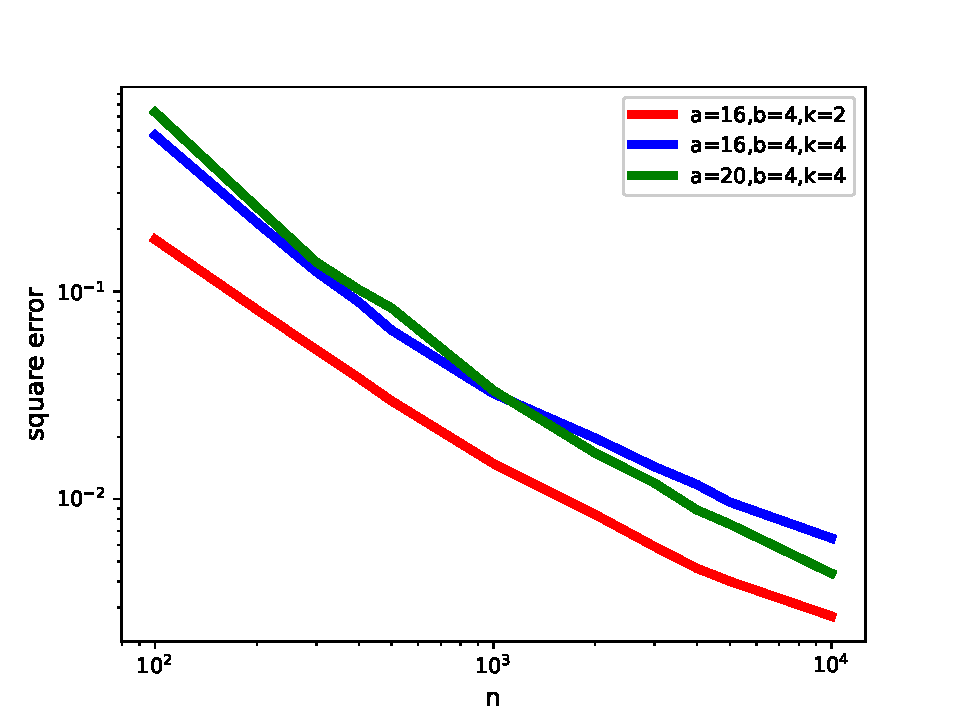
\includegraphics[width=0.6\textwidth]{estimator-error-2020-12-20.pdf}
		\caption{Estimation error of $\hat{a}, \hat{b}$ with respect to $n$.}\label{fig:estimator}
\end{figure}

\section{基于玻茨模型的社群发现算法}
类似于\ref{sec:sibm_model}节
介绍的SIBM模型,我们将
随机块模型
与 \ref{sec:ising} 节介绍的 玻茨模型
复合起来可得到随机块-玻茨模型。该模型可以看成是SIBM模型的推广,
每个节点由两状态变成了多状态。由于我们的研究重点并非
从随机块-玻茨模型的多个样本恢复节点的原始标签,而是利用
玻茨模型对随机块模型进行社群发现,因此我们首先给出
由随机块模型生成的图上定义的玻茨模型:
\begin{definition}\label{def:ising}
	给定从$\SSBM(n,k,\A,\B)$ 中生成的随机图 $G$,
    定义在$G$上的玻茨模型($k$个状态的伊辛模型)带有两个参数 $\gamma,\beta>0$,
	并且是关于状态向量$\sigma\in W^n$ 的概率分布
。该分布的概率质量函数为
\begin{align} \label{eq:isingma}
	P_{\sigma|G}(\sigma=\bar{\sigma})=\frac{\exp(-\beta H(\bar{\sigma}))}{Z_G(\gamma,\beta)}
	\end{align}
其中能量函数$H(\bar{\sigma})$的定义是
\begin{equation}\label{eq:energy}
	H(\bar{\sigma}) := \gamma \frac{\log n}{n} \sum_{\{i,j\}\not\in E(G)} \delta(\bar{\sigma}_i, \bar{\sigma}_j)
	- \sum_{\{i,j\}\in E(G)} \delta(\bar{\sigma}_i, \bar{\sigma}_j)
	\end{equation}
	
	$P_{\sigma|G}$ 中的下标表示该分布依赖于$G$,
    $Z_G(\gamma,\beta)$ 是该分布的归一化常数。
\end{definition}

式\eqref{eq:isingma}中
各符号的含义同式\eqref{eq:canonical_ensemble}。
而表示汉密尔顿能量的式\eqref{eq:energy}
则是式\eqref{eq:ising_modified}的推广。
当  $k=2$ 时 式 \eqref{eq:energy}
在评注\ref{rem:equivalence_H_energy}的意义下
退化成 式 \eqref{eq:ising_modified}。 

这里的能量函数$H(\bar{\sigma})$ 同样有两部分组成:
没有边相连的节点之间排斥力的势能和
有边相连的节点之间吸引力的势能。
$\gamma$ 参数衡量了两种势能之间的比率而
$\frac{\log n}{n}$ 则是对由于边的数量不均匀造成两种势能量阶不同的修正项,
因为两节点间有边相连的概率仅为 $O(\frac{\log n}{n})$。

定义 \ref{def:ising} 实际上给出了一个估计$X$的随机算法 $\hat{X}^*$。
这里,$\hat{X}^*$ 表示产生于玻茨模型的一个样本,
记作$\hat{X}^* \sim \textrm{Potts}_G(\gamma, \beta)$。
沿用评注\ref{rem:metric_exact_recovery} 中的记号,
使用$\hat{X}^*$估计$X$在精确恢复度量下的错误概率
记为 $P_e(\hat{X}^*) := \sum_{G \in \cG_n} P_G(G) P_{\sigma | G}(S^c_k(X))$。
类似定理\ref{thm:sibm_phase_trans}中关于 SIBM 模型的讨论,
玻茨模型的两个参数$(\gamma, \beta)$ 的取值
对$P_e(\hat{X}^*)$
也有着决定性的作用。
当它们取合适的值时, 
$ P_e(\hat{X}^*)\to 0$,
随机块模型的精确恢复可以实现。
反之,如果 $(\gamma, \beta)$ 取其他值时,
$P_e(\hat{X}^*) \to 1$。
这两种情况可总结为如下的定理:

\begin{theorem}\label{thm:phase_transition}
	假设 $\sqrt{a} - \sqrt{b} > \sqrt{k}$,
	定义函数 $g(\beta)$ 和 $ \tilde{g}(\beta)$ 如下:
	\begin{equation}
		\label{eq:g_beta_main_article}
		g(\beta) = \frac{be^{\beta} + a e^{-\beta}}{k} - \frac{a+b}{k} +1
	\end{equation}
	且
	\begin{equation}
		\label{eq:g_tilde_beta_main_article}
	\tilde{g}(\beta) = \begin{cases}
	g(\beta) & \beta \leq \bar{\beta} = \frac{1}{2}\log \frac{a}{b} \\
	g(\bar{\beta}) = 1 - \frac{(\sqrt{a} - \sqrt{b})^2}{k} & \beta > \bar{\beta}
	\end{cases}
	\end{equation}
	其中
	$\bar{\beta} =  \displaystyle\arg\min_{\beta > 0} g(\beta)$。
	令 $\beta^*$ 定义成
	\begin{equation}\label{eq:beta_star}
	\beta^* = \log\left(\frac{a + b - k - \sqrt{(a + b - k)^2 - 4 a b)}}{2  b}\right)
	\end{equation}
	可以验证 $\beta^*$ 是方程 $g(\beta) = 0$ 的解 并且满足  $\beta^* < \bar{\beta}$。
	则取决于 $(\gamma, \beta)$ 如何取值,对于给定的 $\epsilon > 0$, 
	$G\sim \SSBM(n, k, \A, \B)$, $\hat{X}^* \sim \textrm{Potts}_G(\gamma, \beta)$,
	当 $n$ 充分大时, 我们有:
	\begin{enumerate}
	\item 当 $\gamma > b$ 且 $\beta > \beta^*$ 时,$P_e(\hat{X}^*) \leq n^{\tilde{g}(\beta)/2 + \epsilon}$;
	\item 当 $\gamma > b$ 且 $\beta < \beta^*$ 时,$P_a(\hat{X}^*) \leq (1+o(1))\max\{n^{g(\bar{\beta})}, n^{-g(\beta) + \epsilon}\}$;
	\item 当 $\gamma < b$ 时,对于任意给定的 $C>0$	均有 $P_a(\hat{X}^*) \leq \exp(-C n)$。
	\end{enumerate}
\end{theorem}

\begin{figure}[H]
	\begin{subfigure}{0.43\textwidth}
		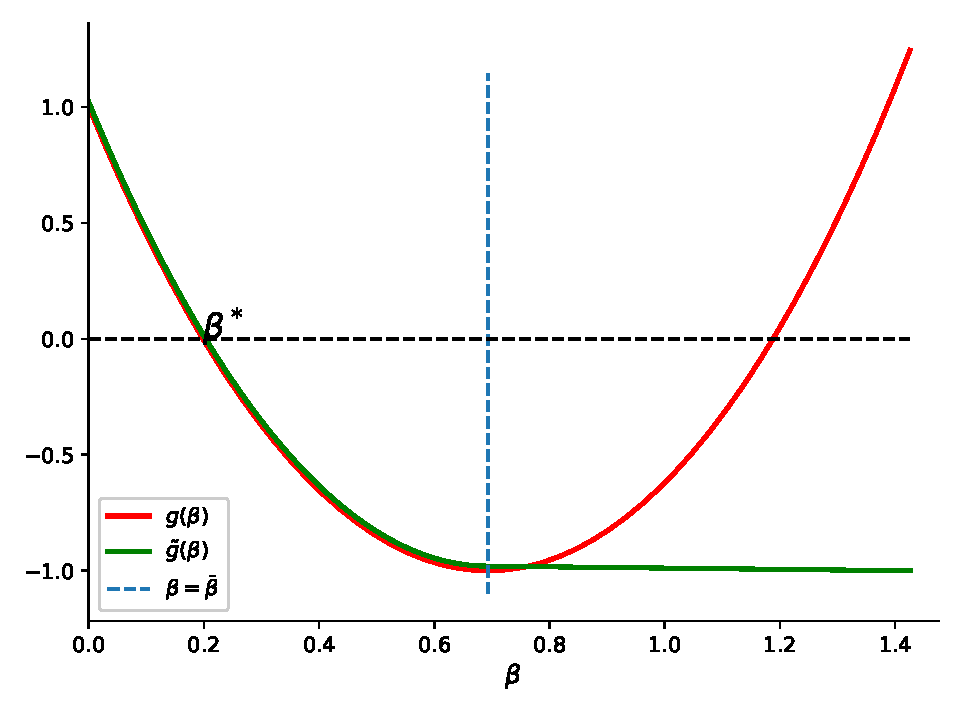
\includegraphics[width=\textwidth]{g-16-4-2.pdf}
		\caption{当 $a=16,b=4,k=2$时,$g(\beta)$和
		$\tilde{g}(\beta)$的函数图像}\label{fig:g}
	\end{subfigure}~
	\begin{subfigure}{0.55\textwidth}
		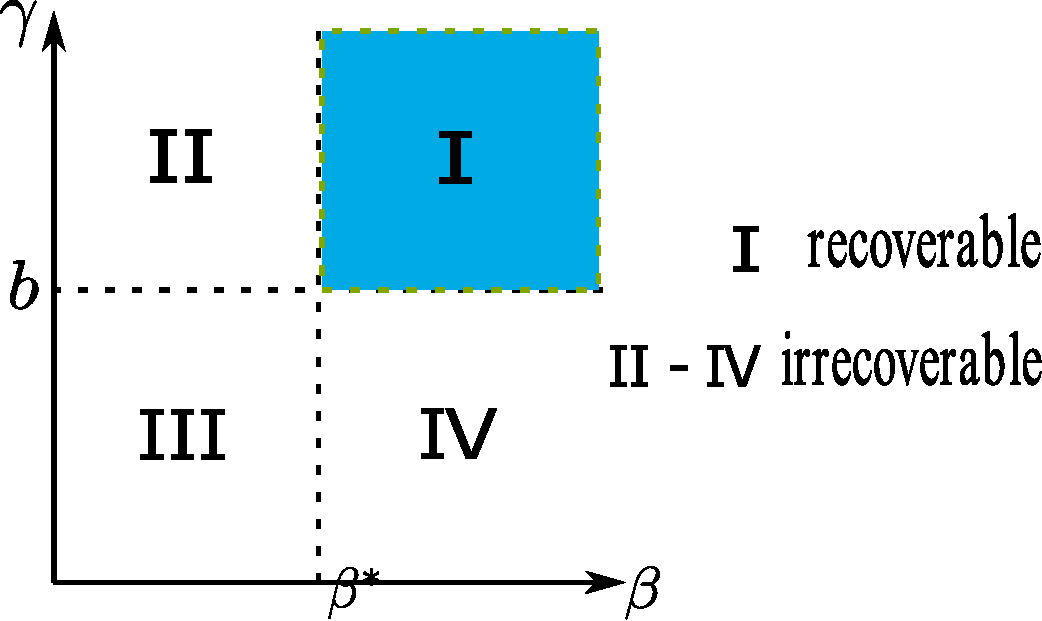
\includegraphics[width=\textwidth]{phase_trans.pdf}
		\caption{
			在 $(\beta, \gamma)$ 平面内
			相变区域图示。
			随机块模型的精确
			恢复仅在区域 I 可实现。}\label{fig:pt}
	\end{subfigure}
	\caption{定理 \ref{thm:phase_transition}
	的图示}
	\label{fig:phase_transition_theorem_illustration}
\end{figure}

与式\eqref{eq:beta_star_sibm}的情形类似,注意到条件$\sqrt{a} - \sqrt{b} > \sqrt{k}$保证了
式\eqref{eq:beta_star}中的根号下的项非负。
这个条件来自于定理\ref{thm:sbmk_phase_transition},
保证了随机块模型本身精确恢复可实现。


通过简单的计算可知,对于 $\beta> \beta^*$ 我们有
$\tilde{g}(\beta) < 0$ 而 对于 $\beta < \beta^*$有
$g(\beta)>0$。
另外,由 $\sqrt{a} - \sqrt{b} > \sqrt{k}$ 可知
$g(\bar{\beta}) < 0$。
$g(\beta), \tilde{g}(\beta)$ 的图像
如图 \ref{fig:phase_transition_theorem_illustration}a 所示。
因此, 对于充分小的
$\epsilon$ 并且当 $n \to \infty$,
定理\ref{thm:phase_transition} 中给出的上界
均至少以多项式的速度趋向于 $0$。
从而定理\ref{thm:phase_transition} 
刻划了
玻茨模型的相变性质。
如图\ref{fig:phase_transition_theorem_illustration}b所示
, 对于玻茨模型, 只有参数$(\beta, b)$落在区域I时,
随机块模型的精确
恢复才能实现。

定理\ref{thm:phase_transition}
也可以从$\sigma$的边缘分布的角度理解。
玻茨模型取到某个特定状态$\bar{\sigma}$的概率为
 $\sigma: P_{\sigma}(\sigma =\bar{\sigma})
=\sum_{G \in \cG_n}P_G(G)P_{\sigma |G}(\sigma=\bar{\sigma})$.
\newglossaryentry{not:sigma_nearest_to_the_latter}
{
  type=notation,
  name={\ensuremath{D(\sigma, \sigma')}},
  description={$\sigma$ 相比于它的所有置换其本身离 $\sigma'$ 最近
  这个事件}
}
我们用符号 \gls{not:sigma_nearest_to_the_latter} 表示 \glsdesc{not:sigma_nearest_to_the_latter}
。
也即
\begin{equation}
	\label{eq:D_sigma_sigma_prime}
D(\sigma, \sigma') := \{ \sigma = \arg\min_{f \in S_k} \Dist(f(\sigma), \sigma')  \}
\end{equation}

则 定理 \ref{thm:phase_transition} 
对边缘分布 $P_{\sigma}$ 蕴含着如下的论断
:
\begin{corollary}\label{cor:phase4}
假设 $\gamma > b$, 取决于 $\beta$ 的取值我们有
\begin{enumerate}
	\item 当 $\beta > \beta^*$时,$P_{\sigma}(\sigma = X | D(\sigma, X))  = 1-o(1)$;
	\item 当 $\beta < \beta^*$时,$P_{\sigma}(\sigma = X | D(\sigma, X))  = o(1)$。
\end{enumerate}
\end{corollary}

下面我们简单阐述下 定理 \ref{thm:phase_transition} 证明的思路。
该思路主要通过对翻转一个状态的前后能量差的分析来估计概率的主项。
下面的引理总结了翻转一个状态汉密尔顿能量的变化:
\begin{lemma}\label{lem:lemmaDiff}
	假设 $\bar{\sigma}'$ 仅在第$r$个位置上与 $\bar{\sigma}$ 不同,
	差别为 $\bar{\sigma}'_r = \omega^s \cdot \bar{\sigma}_r$。
	则 $\bar{\sigma}'$ 和 $\bar{\sigma}$ 的能量差为
\begin{align}
	H(\bar{\sigma}') - H(\bar{\sigma}) &= (1+\gamma \frac{\log n}{n})\sum_{i \in N_r(G)} J_s(\bar{\sigma}_r, \bar{\sigma}_i)
	\notag \\
	&+ \gamma \frac{\log n}{n} (m(\omega^s \cdot \bar{\sigma}_r)-m(\bar{\sigma}_r)+1) \label{eq:DeltaH}
	\end{align}
	上式中 $m(\omega^j) := |\{i \in [n] | \bar{\sigma}_i = \omega^j | \}$, $N_r(G):=\{j | (r, j) \in E(G) \}$ 且 $J_s(x, y) = \delta(x, y) - \delta(\omega_s \cdot x, y)$.
\end{lemma}
引理 \ref{lem:lemmaDiff} 提供了用以比较两个相邻状态的    概率
的方法,即:
\begin{equation}\label{eq:Pratio}
\frac{P_{\sigma |G } (\sigma = \bar{\sigma}')}{P_{\sigma |G } (\sigma = \bar{\sigma})}
= \exp(-\beta(H(\bar{\sigma}') - H(\bar{\sigma})))
\end{equation}

另外, 我们注意到 因为图的边的数量是稀疏的,每个节点
平均有 $O(\log n)$ 个相连的邻居节点。
按照式 \eqref{eq:DeltaH} 
计算能量差的时间复杂度也是 $O(\log n)$。

当 $H(\bar{\sigma}') > H(\bar{\sigma})$ 时, 
由式\eqref{eq:Pratio} 可得
$P_{\sigma | G}(\sigma = \bar{\sigma}')$
小于
$P_{\sigma | G}(\sigma = \bar{\sigma})$。
粗略而言, 如果
$ \sum_{\Dist(\sigma', X)=1}\exp(-\beta(H(\bar{\sigma}') - H(X))) $
收敛到零,
我们可以预期,与$S_k(X)$不同的所有其他状态的概率收敛到零。
与之相反, 如果
$ \sum_{\Dist(\sigma', X)=1}\exp(-\beta(H(\bar{\sigma}') - H(X))) $
趋于无穷大,
则 $P_{\sigma}(S_k(X))$ 趋于零。
此种分析展示了证明定理 \ref{thm:phase_transition}的
主要思路。
严格的证明参见附录 \ref{sec:appendix_theorem_proof_phase_trans}。

\section{通过能量最小化进行社群发现}\label{sec:em}
因为 $\beta^*$ 和 $n$ 无关,
当 $\gamma>b$ 时,
我们可以选取一个足够大的 $\beta$ 使得
$\beta > \beta^*$,
则 由 定理\ref{thm:phase_transition}, 当$n$充分大时 $\sigma \in S_k(X)$ 几乎必然发生。
这蕴含了 $P_{\sigma | G}(\sigma = X)$
对于几乎所有的 从 SBM 采样的图  $G$来说 取得最大值。
因此
相比于从伊辛模型中采样的方法,我们可以直接最大化条件概率,以
找到概率最大值的状态。
等价地, 我们可以通过最小化 \eqref{eq:energy}式的方式来获得状态的估计量:
\begin{equation}\label{eq:hatX}
\hat{X}' := \arg\min_{\bar{\sigma} \in W^n} H(\bar{\sigma})
\end{equation}

在 \eqref{eq:hatX} 中, 我们让 $\bar{\sigma}$ 在 $W^n$ 中取值。
因为我们已知 $X$取各个标签的位置数相等,即对于每个标签值 $u$
有 $|\{v \in [n] : X_v = u\}| = \frac{n}{k}$,
我们可以把搜索空间限制到
$W^*:= \{\sigma\in W^n \big\vert |\{v \in [n] : \sigma_v = \omega^s\}| = \frac{n}{k}, s=0,\dots, k-1 \}$
上。
当 $\sigma \in W^*$ 时, 最小化 $H(\sigma)$ 等价于:
\begin{equation}\label{eq:hatX_double_prime}
\hat{X}'' := \arg\min_{\sigma \in W^*} \sum_{\{i,j\} \not\in E(G) } \delta(\sigma_i, \sigma_j)
\end{equation}
其中最小值是不同社群之间的最小分割。

当 $\hat{X}'' \neq X$ 时,
我们必须有  $\Dist(\hat{X}'' ,X)\geq 2$
以满足 硬约束 $\hat{X}'' \in W^*$。
此外,估计量 $\hat{X}''$ 是无参的而 $\hat{X}'$的值受
参数 $\gamma$ 的影响。
在
$\hat{X}'$ 的表达式中出现的额外的参数 $\gamma$ 可视为
某种整数规划的拉格朗日乘子。
因此,通过引入惩罚因子项和将搜索空间从$W^*$ 扩大 到$W^n$
,求解 $\hat{X}'$
的优化问题 转变为 $\hat{X}''$的优化问题。

当 $\beta > \bar{\beta}$ 时,
$\tilde{g}(\beta)$ 是一个常数。
因此,从 Theorem \ref{thm:phase_transition} 中我们可以获得的关于
伊辛模型的估计量 $\hat{X}^*$ 最紧的上界
是  $n^{g(\bar{\beta})/2}$。

对于 $\hat{X}'$ 和 $\hat{X}''$ 这两个估计量,
我们可以获得 更紧的误差上界。我们把这一结果总结为如下定理:
\begin{theorem}\label{thm:error_rate}
当 $\sqrt{a} - \sqrt{b} > \sqrt{k}$ 时,
对于充分大的 $n$,我们有 
\begin{enumerate}
	\item 若 $\gamma > b$, $P_G(\hat{X}' \not\in S_k(X)) \leq (k-1+o(1))n^{g(\bar{\beta})}$;
	\item $P_G(\hat{X}'' \not\in S_k(X)) \leq ((k-1)^2+o(1))n^{2g(\bar{\beta})}$。
\end{enumerate}
\end{theorem}
因为 $g(\bar{\beta})<0$, 我们有大小关系 $n^{2g(\bar{\beta})} < n^{g(\bar{\beta})} < n^{g(\bar{\beta})/2}$。
从而 定理 \ref{thm:error_rate} 说明了在三个估计量中,
$P_e(\hat{X}'')$ 
的上界最紧。
这可以直观地理解为搜索空间缩小的结果。
定理\ref{thm:error_rate} 的证明技术是对于 $\Dist(\bar{\sigma}, X) \geq 1$,考虑事件
$H(X) > H(\bar{\sigma})$发生的概率。
然后通过布尔不等式, 这些概率可以相加。
关于估计量 $\hat{X}''$ 误差上界的研究早在\citet{abbe2015exact} 的工作中即有涉及,
但他只得到了一个比较松的上界 $n^{g(\bar{\beta})/4}$,且仅针对 $k=2$ 的情形。
对于一般的情形,
当条件
$\sqrt{a} - \sqrt{b} > \sqrt{k}$ 满足时,考虑到
$\tilde{g}(\beta) = 1- \frac{(\sqrt{a} - \sqrt{b})^2}{k}$,
定理 \ref{thm:error_rate} 说明了  $\hat{X}'$ 和 $\hat{X}''$
均可实现
精确恢复。


估计量 $\hat{X}'$ 有一个参数 $\gamma$。
当 $\gamma$ 取特定的值时, $\hat{X}'$在渐近情形下
可以等价于 最大似然估计或最大模块度估计。
以下分析从直观地角度说明了
这种联系。

通过最大化对数似然函数可得到最大似然估计量。
由 \eqref{eq:GmL} 式,该似然函数可以进一步写成:
\begin{equation}\label{eq:PG_energy}
	\log P_G(Z=z|X=\sigma) = -\log\frac{a}{b} \cdot H(\sigma) + C
\end{equation}

这里 在$H(\sigma)$ 的表达式中 参数 $\gamma$ 的取值满足
\begin{equation}\label{eq:special_gamma_ML}
	\gamma \frac{\log n}{n} = \frac{1}{\log(a/b)}
	\left(\log (1-\B) - \log (1-\A) \right)	 
\end{equation}

而 $C$ 是一个和 $\sigma$ 无关的常数。
当 $n$ 充分大时,我们有 $\gamma \to \gamma_{ML} := \frac{a-b}{\log(a/b)}$。   
也即,
当 $\gamma = \gamma_{ML}$时,
最大似然估计量 渐近等价于 $\hat{X}'$。

这里我们顺便得到了最大似然算法和最小割问题在有$W^*$约束
下的等价性,这个等价性不需要渐近的条件也成立。
因为最大似然算法首先等价于极小化能量$H(\sigma)$,
$\gamma$从\eqref{eq:special_gamma_ML}式中取值。其次,
由\eqref{eq:hatX_double_prime}式,极小化能量$H(\sigma)$
等价于$\min \sum_{\{i,j\} \not\in E(G) } \delta(\sigma_i, \sigma_j)$
因为在$W^*$的约束下,
$\sum_{1<i<j<n} \delta(\sigma_i, \sigma_j)$
是一个常数,\eqref{eq:hatX_double_prime}式又等价于
$-\sum_{ \{i,j\} \in E} \delta(\sigma_i, \sigma_j)$,
其与 \eqref{eq:minimum_k_cut}式只相差一个常数。


最大模块度估计量通过最大化 \ref{eq:Q}式而得到。
忽略常数项,关于标签向量 $\sigma$的模块度 $Q$
可以写成:
\begin{align}
Q(\sigma) = -\sum_{\{i,j\} \not\in E(G) } \frac{d_i d_j}{2 |E|}\delta(\sigma_i,\sigma_j) 
+ \sum_{\{i,j\} \in E(G) } (1 - \frac{d_i d_j}{2 |E|}) \delta(\sigma_i,\sigma_j)  \label{eq:Qtransform}
\end{align}

当$n$充分大时,平均意义上我们有 $d_i \sim  \frac{(a+(k-1)b)\log n}{k}, |E| \sim \frac{1}{2}n d_i$。
因此,我们有
$\frac{d_id_j}{2|E|} \to \gamma_{MQ} \frac{\log n}{n} $。
从 \eqref{eq:Qtransform}式我们可以看到,
当 $\gamma = \gamma_{MQ} = \frac{a+(k-1)b}{k}$ 且 $n\to \infty$时,
$Q(\sigma) \to -H(\sigma)$。
也即,当$\gamma = \gamma_{MQ}$ 时,
最大模块度估计量渐近等价于
$\hat{X}'$ 。


通过$a>b$和 当$x>1$时的不等式 
 $x-1>\log x $,我们可以验证
  $\gamma_{MQ} >b$ 且  $\gamma_{ML} > b$。
  这说明 了
  最大似然估计和最大模块度估计都满足
  定理\ref{thm:error_rate}所述的精确恢复条件 $\gamma > b $。

\section{基于梅特罗波利斯算法的社群发现}\label{sec:ms}

由定理\ref{thm:phase_transition}可知,
如果我们直接从玻茨模型 \eqref{eq:isingma} 式中采样,那么得到的样本大概率
与$X$一致。
然而,当$n$非常大时,按照分布\eqref{eq:isingma}式精确采样是困难的,
因为状态空间的状态总数随着$n$以
$k^n$的速率指数增大。
因此,一定程度的近似是必要的,
为此我们可以借助 \ref{sec:ising} 节介绍的梅特罗波利斯算法。 
经过若干次初始迭代后,梅特罗波利斯算法
每次产生的样本可视为从玻茨模型 采样的结果。
这个论断相关的理论研究主要是基于马尔可夫链。
在某些一般性的条件下,
梅特罗波利斯算法生成的样本收敛到
马尔可夫链的稳态并且该稳态分布即为要近似的分布。
针对伊辛模型的不同变体,
之前的许多工作都表明了梅特罗波利斯算法采样的收敛性\cite{diaconis1998we}。
这里我们假设可以推广类似的收敛性结果可以推广到
形如 \eqref{eq:isingma} 式中描述的玻茨模型。

我们对算法 \ref{alg:Metropolis}
进行改写即可得到针对我们的模型和能量表达式 \eqref{eq:energy},
的算法 \ref{alg:m}。
算法 \ref{alg:m} 要求
社群数量 $k$ 和参数 $\beta, \gamma$ 事先给定。
并且,根据定理\ref{thm:phase_transition},我们需选取  $\beta>\beta^*, \gamma > b$
\footnote{ $\beta^*$ 的定义参见式 \eqref{eq:beta_star} }
。
这里的 $a, b$
可以通过 定理 \ref{thm:ab12} 中提出的估计量$\hat{a},\hat{b}$进行近似。
此外,算法的迭代次数  $N$
也需事先确定。
\begin{algorithm}[H]
	\caption{针对玻茨模型的梅特罗波利斯算法} \label{alg:m}
	输入: 图 $G$, 参数 $\beta$、$\gamma$ \\
	输出: $\hat{X} = \bar{\sigma}$
	\begin{algorithmic}[1]
		\STATE 随机初始化 $\bar{\sigma} \in W^n$ %\vskip 0.5em
		\FOR{$i=1,2,\dots, N$}
		\STATE 根据引理 \ref{lem:lemmaDiff},
		随机选取 $s, r$ 并得到新的状态
		 $\bar{\sigma}'$
		 %\vskip 0.5em
		\STATE 通过 \eqref{eq:DeltaH} 计算 $\Delta H(r,s) = H(\bar{\sigma}') - H(\bar{\sigma})$ %\vskip 0.5em
		\IF{$\Delta H(r,s)<0$}
		\STATE $\sigma_r \leftarrow w^s \cdot \sigma_r$ %\vskip 0.5em
		\ELSE
		\STATE 以概率 $\exp(-\beta \Delta H(r,s))$ 使得
			$\sigma_r \leftarrow w^s \cdot \sigma_r$,
			否则保持原状。 %\vskip 0.5em
		\ENDIF %\vskip 0.5em
		\ENDFOR
	\end{algorithmic}
\end{algorithm}
 由 引理 \ref{lem:lemmaDiff} , $\Delta H(r,s)$ 的计算需要 $O(\log n)$ 的时间。
有研究针对某种特殊的伊辛模型指出
$N=O(n\log n)$ 即可得到估计得比较好的样本\cite{mcmc}。
对于我们的模型,由于我们并不清楚 $ N = O(n\log n)$ 是否足够,
因此我们在数值实验中经验地选取 $N=O(n^2)$。
则 算法 \ref{alg:m} 总的时间复杂度为 $O(n^2 \log n)$。



借助梅特罗波利斯算法,
下面我们通过实验验证 定理 \ref{thm:phase_transition} 中的 $\gamma > b$的情形。
我们选取了 $n=9000, k=2$,
通过蒙特卡罗采样的方法,我们可以得到准确率的经验计算公式为
$P_a(\hat{X}^*) = \frac{1}{m_1m_2}\sum_{i=1}^{m_1} \sum_{j=1}^{m_2} \mathbf{1}[\hat{X}^* = \pm X]$。
在这个公式中,
$m_1$ 是 由 SBM 模型产生的随机图的次数,而
$m_2$ 是 对于一个特定的图,由算法\ref{alg:m} 生成的连续样本的数量。
我们选取 $m_1=2100,m_2=6000$。这样的取值已相当大,
且由大数定律
可达到 $P_a(\hat{X}^*)$ 的好的估计。
$P_a(\hat{X}^*)$ 随 $\beta$的变化在 图 \ref{fig:erh}
中给出。

\begin{figure}[ht!]
	\centering
		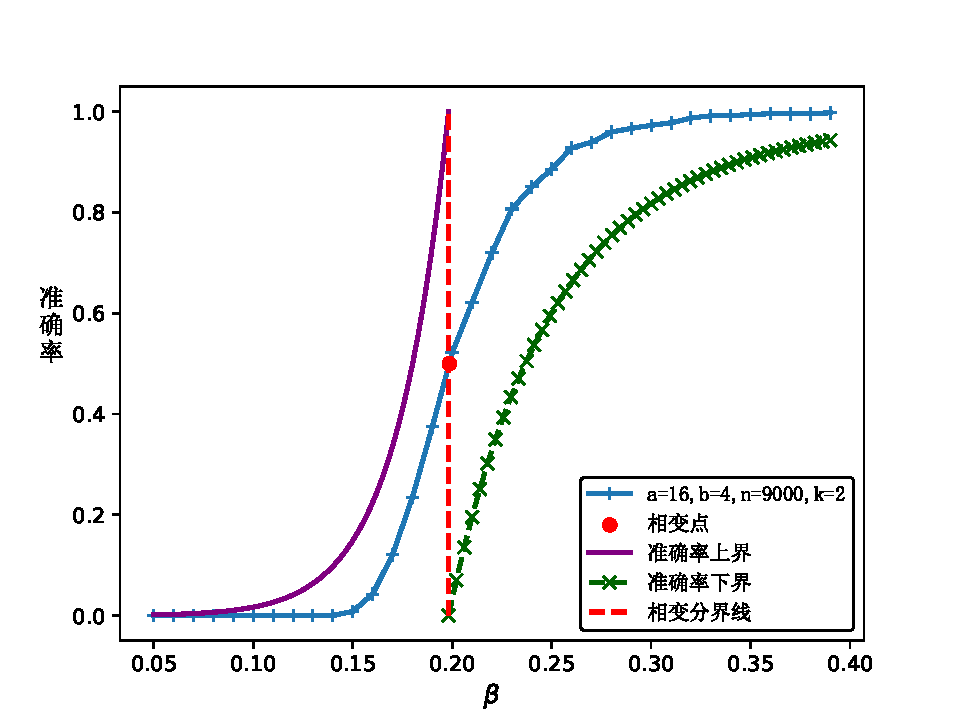
\includegraphics[width=0.6\textwidth]{beta_trans-2020-11-28.pdf}
		\caption{使用 $\hat{X}^*$ 进行社群发现精确恢复的准确率}\label{fig:erh}
\end{figure}


竖线 ($\beta=\beta^* \approx 0.198$),
是 从 \eqref{eq:beta_star} 式计算得到的, 
代表了相变的临界值。
图 \ref{fig:erh}中的坐标点 $(0.199,\frac{1}{2})$
可视为通过实验估计出的
相变点,它的横坐标接近
$\beta^*$。
绿线 $(\beta, n^{g(\beta)/2})$ 
表示当 $\beta>\beta^*$ 时准确率的理论下界,
而紫线
$(\beta, n^{-g(\beta)})$ 
表示当 $\beta<\beta^*$ 时准确率的理论上界。
仿真实验得到的相变曲线(蓝线)恰好介于此两线之间。
当 $n$ 变得更大时,可预见
相变曲线 将接近阶跃函数,该函数的值在
$\beta=\beta^*$ 处
从 0 跳变到 1。
